\newpage
\section{Description of Models}
\todo[inline]{This section shall describe your models for the different subsystems for the two architectures and the two levels of functionality. Figures should be explained in the text.}

In this section, models for the two architectures and their subsystems will be described.

\subsection{Wheel Unit Model}
Each wheel unit consists of three different components, sensors (S), actuator (A), and computing modules (CM), organized as in \figref{fig2}. There are two redundant CMs, two redundant sensors, and one actuator, yielding the reliability block diagram shown in \figref{fig3}.   
\begin{figure}[H]
  \centering
  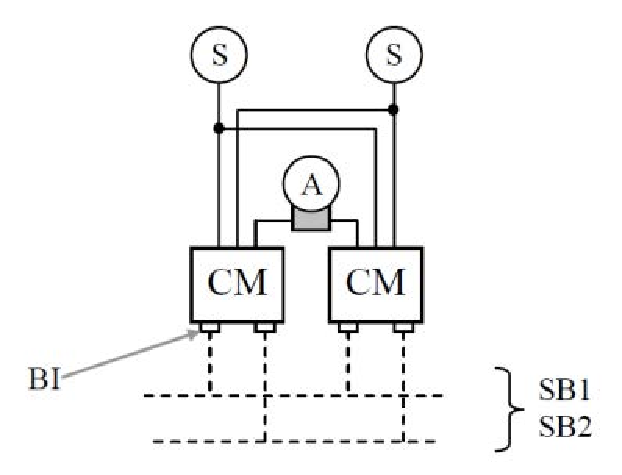
\includegraphics[scale=0.7]{Fig2.pdf}
  \caption{Wheel Unit}
  \label{fig2}
\end{figure}
\begin{figure}[H]
  \centering
  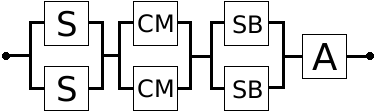
\includegraphics[scale=0.7]{wu_block.png}
  \caption{Reliability block diagram of the wheel unit}
  \label{fig3}
\end{figure}
%--------------------------------
\subsection{Wheel Unit Subsystem Model}
The combination of all four WUs yields the wheel unit subsystem. In the full functionality mode of operation the subsystem can not tolerate any broken WUs, for which a fault tree is shown in \figref{fig4}. When running in the other mode of operation, allowing degraded functionality, one WU can become faulty without causing a full system failure, shown in \figref{fig5}. 
\begin{figure}[H]
  \centering
  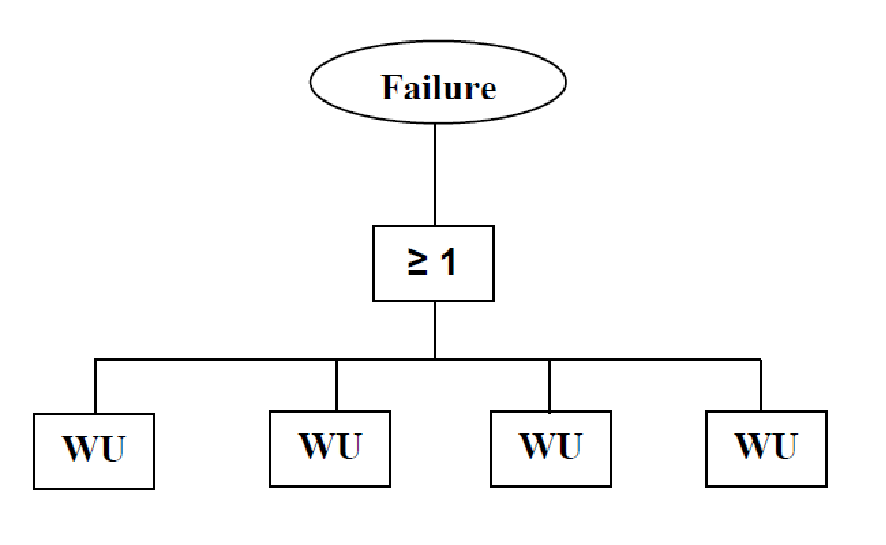
\includegraphics[scale=0.5]{Fig4.pdf}
  \caption{Fault tree for the Wheel Unit Subsystem, full functionality}
  \label{fig4}
\end{figure}
\begin{figure}[H]
  \Tree[.{WU Failure} [.{$2 \geq$} WU WU WU WU ] ]
  \caption{Fault tree for the Wheel Unit Subsystem, degraded functionality}
  \label{fig5}
\end{figure}
%--------------------------------
\subsection{Central Unit (CU)}
In the two evaluated architectures the central unit is configured in two different ways. The central unit for the distributed architecture is described in \secref{subsec:dda} and the central unit for the centralized architecture is described in \secref{subsec:cta}. 

\subsubsection{Distributed Duplex Architecture}
\label{subsec:dda}
The distributed architecture's central unit consists of two computing modules (CM) configured in duplex. Each CM fails silent with a coverage factor of $99\%$. If a violation of the fail-silent property occurs, i.e. a CM delivers a erroneous result, the central unit fails. In \figref{fig6}

\begin{figure}
  \centering
  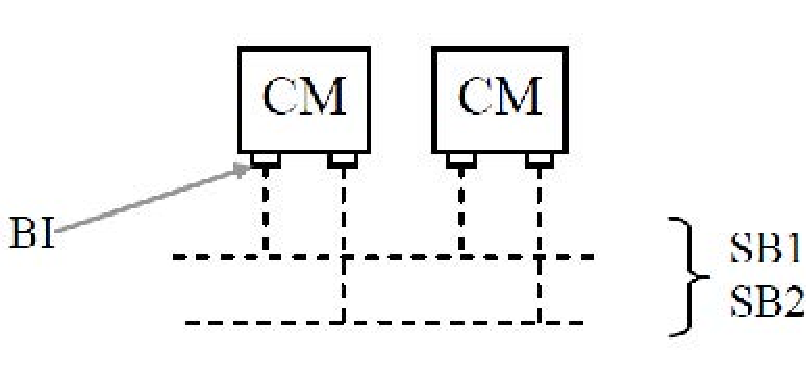
\includegraphics[scale=.5]{Fig6.pdf}
  \caption{Central Unit, duplex configuration }
  \label{fig6}
\end{figure}
\begin{figure}[H]
  \centering
  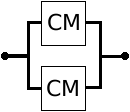
\includegraphics[scale=1.0]{cm2_block.png}
  \caption{Reliability block diagram for the Central Unit, duplex configuration}
  \label{fig7}
\end{figure}
\begin{figure}[h!]
  \begin{center}
    \begin{tikzpicture}[node distance=5mm and 20mm]
      \node[state] (s2) {A};
      \node[state] (s3) [right= of s2] {B};
      \node[state] (s4) [right= of s3] {C};
      \draw [->,bend left=45] (s2) to node[above] {$c*2\lambda_{CU-CM} $} (s3);
      \draw [->,bend right=45] (s2) to node[below] {$(1-c)*2\lambda_{CU-CM}$} (s4);
      \draw [->,bend left=45] (s3) to node[above] {$\lambda_{CU-CM}$} (s4);
    \end{tikzpicture}
  \caption{Markov chain model}
\end{center}
\end{figure}
%-------------
\subsubsection{Centralized Triplex Architecture}
\label{subsec:cta}
\begin{figure}[H]
  \centering
  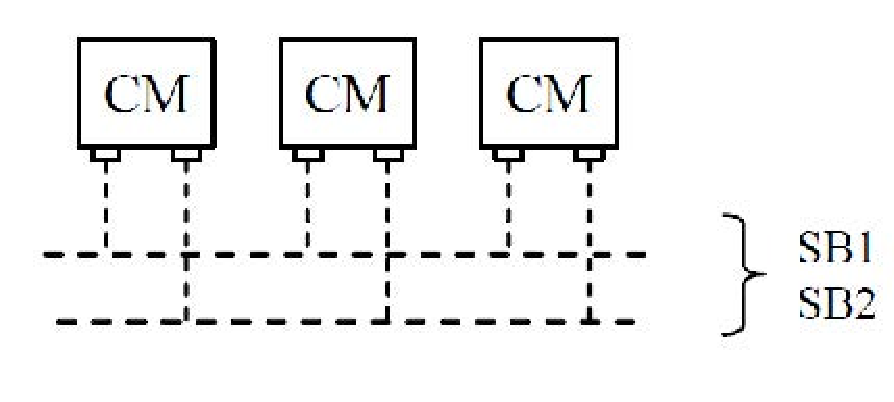
\includegraphics[scale=.5]{Fig9.pdf}
  \caption{Central Unit, triplex configuration }
  \label{fig9}
\end{figure}
/{Reliability block diagram for …, Figure 10.  Make sure the caption number is correct.}/
\\/{Markov model for …, Figure 11.}/

\begin{figure}[H]
  \centering
  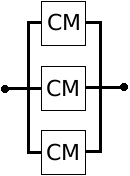
\includegraphics[scale=.5]{cm3_block.png}
  \caption{Caption }
  \label{fig10}
\end{figure}
\begin{figure}[H]
  \centering
  \begin{tikzpicture}[node distance=5mm and 20mm]
    \node[state] (sa) {3};
    \node[state] (sb) [right= of sa] {2};
    \node[state] (sc) [right= of sb] {1};
    \node[state] (sd) [right= of sc] {F};
    \draw [->,bend left=45] (sa) to node[above] {$3\lambda_{CU-CM} $} (sb);
    \draw [->,bend left=45] (sb) to node[above] {$c*2\lambda_{CU-CM} $} (sc);
    \draw [->,bend right=45] (sb) to node[below] {$(1-c)*2\lambda_{CU-CM}$} (sd);
    \draw [->,bend left=45] (sc) to node[above] {$\lambda_{CU-CM}$} (sd);
  \end{tikzpicture}
  \caption{Caption}
  \label{fig11}
\end{figure}
%--------------------------------
\subsection{System Model}
\subsubsection{Centralized Architecture}

\begin{figure}[H]
  \Tree[.{System Failure} [.{$1 \geq$} [.{CU subsystem fail} [.{$2 \geq$} CM CM CM ] ] [.{WU subsystem fail} [.{$1 \geq$} WU WU WU WU ] ] [.{SB subsystem fail} [.{\&} SB SB ] ] ] ]
  \caption{Fault tree for Full Functionality}
  \label{fig12}
\end{figure}
\begin{figure}[H]
  \Tree[.{System Failure} [.{$1 \geq$} [.{CU subsystem fail} [.{$2 \geq$} CM CM CM ] ] [.{WU subsystem fail} [.{$2 \geq$} WU WU WU WU ] ] [.{SB subsystem fail} [.{\&} SB SB ] ] ] ]
  \caption{Fault tree for Degraded Functionality}
  \label{fig13}
\end{figure}
%-------------
\subsubsection{Distributed Architecture}
\begin{figure}[H]
  \Tree[.{System Failure} [.{$1 \geq$} [.{CU subsystem fail} [.{$1 \geq$} CM CM ] ] [.{WU subsystem fail} [.{$1 \geq$} WU WU WU WU ] ] [.{SB subsystem fail} [.{\&} SB SB ] ] ] ]
  \caption{Fault tree for Full Functionality}
  \label{fig14}
\end{figure}
\begin{figure}[H]
  \Tree[.{System Failure} [.{$1 \geq$} [.{CU subsystem fail} [.{$1 \geq$} CM CM ] ] [.{WU subsystem fail} [.{$2 \geq$} WU WU WU WU ] ] [.{SB subsystem fail} [.{\&} SB SB ] ] ] ]
  \caption{Fault tree for Degraded Functionality}
  \label{fig15}
\end{figure}